% GNUPLOT: LaTeX picture with Postscript
\begingroup
  \makeatletter
  \providecommand\color[2][]{%
    \GenericError{(gnuplot) \space\space\space\@spaces}{%
      Package color not loaded in conjunction with
      terminal option `colourtext'%
    }{See the gnuplot documentation for explanation.%
    }{Either use 'blacktext' in gnuplot or load the package
      color.sty in LaTeX.}%
    \renewcommand\color[2][]{}%
  }%
  \providecommand\includegraphics[2][]{%
    \GenericError{(gnuplot) \space\space\space\@spaces}{%
      Package graphicx or graphics not loaded%
    }{See the gnuplot documentation for explanation.%
    }{The gnuplot epslatex terminal needs graphicx.sty or graphics.sty.}%
    \renewcommand\includegraphics[2][]{}%
  }%
  \providecommand\rotatebox[2]{#2}%
  \@ifundefined{ifGPcolor}{%
    \newif\ifGPcolor
    \GPcolortrue
  }{}%
  \@ifundefined{ifGPblacktext}{%
    \newif\ifGPblacktext
    \GPblacktexttrue
  }{}%
  % define a \g@addto@macro without @ in the name:
  \let\gplgaddtomacro\g@addto@macro
  % define empty templates for all commands taking text:
  \gdef\gplbacktext{}%
  \gdef\gplfronttext{}%
  \makeatother
  \ifGPblacktext
    % no textcolor at all
    \def\colorrgb#1{}%
    \def\colorgray#1{}%
  \else
    % gray or color?
    \ifGPcolor
      \def\colorrgb#1{\color[rgb]{#1}}%
      \def\colorgray#1{\color[gray]{#1}}%
      \expandafter\def\csname LTw\endcsname{\color{white}}%
      \expandafter\def\csname LTb\endcsname{\color{black}}%
      \expandafter\def\csname LTa\endcsname{\color{black}}%
      \expandafter\def\csname LT0\endcsname{\color[rgb]{1,0,0}}%
      \expandafter\def\csname LT1\endcsname{\color[rgb]{0,1,0}}%
      \expandafter\def\csname LT2\endcsname{\color[rgb]{0,0,1}}%
      \expandafter\def\csname LT3\endcsname{\color[rgb]{1,0,1}}%
      \expandafter\def\csname LT4\endcsname{\color[rgb]{0,1,1}}%
      \expandafter\def\csname LT5\endcsname{\color[rgb]{1,1,0}}%
      \expandafter\def\csname LT6\endcsname{\color[rgb]{0,0,0}}%
      \expandafter\def\csname LT7\endcsname{\color[rgb]{1,0.3,0}}%
      \expandafter\def\csname LT8\endcsname{\color[rgb]{0.5,0.5,0.5}}%
    \else
      % gray
      \def\colorrgb#1{\color{black}}%
      \def\colorgray#1{\color[gray]{#1}}%
      \expandafter\def\csname LTw\endcsname{\color{white}}%
      \expandafter\def\csname LTb\endcsname{\color{black}}%
      \expandafter\def\csname LTa\endcsname{\color{black}}%
      \expandafter\def\csname LT0\endcsname{\color{black}}%
      \expandafter\def\csname LT1\endcsname{\color{black}}%
      \expandafter\def\csname LT2\endcsname{\color{black}}%
      \expandafter\def\csname LT3\endcsname{\color{black}}%
      \expandafter\def\csname LT4\endcsname{\color{black}}%
      \expandafter\def\csname LT5\endcsname{\color{black}}%
      \expandafter\def\csname LT6\endcsname{\color{black}}%
      \expandafter\def\csname LT7\endcsname{\color{black}}%
      \expandafter\def\csname LT8\endcsname{\color{black}}%
    \fi
  \fi
    \setlength{\unitlength}{0.0500bp}%
    \ifx\gptboxheight\undefined%
      \newlength{\gptboxheight}%
      \newlength{\gptboxwidth}%
      \newsavebox{\gptboxtext}%
    \fi%
    \setlength{\fboxrule}{0.5pt}%
    \setlength{\fboxsep}{1pt}%
\begin{picture}(14400.00,5040.00)%
    \gplgaddtomacro\gplbacktext{%
      \csname LTb\endcsname%%
      \put(444,440){\makebox(0,0)[r]{\strut{}\np{10}}}%
      \put(444,1509){\makebox(0,0)[r]{\strut{}\np{e2}}}%
      \put(444,2579){\makebox(0,0)[r]{\strut{}\np{e3}}}%
      \put(444,3648){\makebox(0,0)[r]{\strut{}\np{e4}}}%
      \put(444,4717){\makebox(0,0)[r]{\strut{}\np{e5}}}%
      \put(576,220){\makebox(0,0){\strut{}$0$}}%
      \put(2336,220){\makebox(0,0){\strut{}$5$}}%
      \put(4095,220){\makebox(0,0){\strut{}$10$}}%
    }%
    \gplgaddtomacro\gplfronttext{%
      \csname LTb\endcsname%%
      \put(-172,2739){\rotatebox{-270}{\makebox(0,0){\strut{}$\nu_\tau$/cm\tapi{2}/GeV}}}%
      \put(2687,-110){\makebox(0,0){\strut{}Energy (GeV)}}%
      \csname LTb\endcsname%%
      \put(4182,4844){\makebox(0,0)[r]{\strut{}0 MeV}}%
      \csname LTb\endcsname%%
      \put(4182,4580){\makebox(0,0)[r]{\strut{}100 MeV}}%
      \csname LTb\endcsname%%
      \put(4182,4316){\makebox(0,0)[r]{\strut{}150 MeV}}%
      \csname LTb\endcsname%%
      \put(4182,4052){\makebox(0,0)[r]{\strut{}180 MeV}}%
      \csname LTb\endcsname%%
      \put(4182,3788){\makebox(0,0)[r]{\strut{}190 MeV}}%
    }%
    \gplgaddtomacro\gplbacktext{%
      \csname LTb\endcsname%%
      \put(5820,440){\makebox(0,0)[r]{\strut{}0.8}}%
      \put(5820,1590){\makebox(0,0)[r]{\strut{}0.85}}%
      \put(5820,2740){\makebox(0,0)[r]{\strut{}0.9}}%
      \put(5820,3889){\makebox(0,0)[r]{\strut{}0.95}}%
      \put(5820,5039){\makebox(0,0)[r]{\strut{}1}}%
      \put(5952,220){\makebox(0,0){\strut{}$0$}}%
      \put(6936,220){\makebox(0,0){\strut{}$0.5$}}%
      \put(7920,220){\makebox(0,0){\strut{}$1$}}%
      \put(8903,220){\makebox(0,0){\strut{}$1.5$}}%
      \put(9887,220){\makebox(0,0){\strut{}$2$}}%
    }%
    \gplgaddtomacro\gplfronttext{%
      \csname LTb\endcsname%%
      \put(5072,2739){\rotatebox{-270}{\makebox(0,0){\strut{}Factor}}}%
      \put(7919,-110){\makebox(0,0){\strut{}Mass (GeV)}}%
      \csname LTb\endcsname%%
      \put(9270,4844){\makebox(0,0)[r]{\strut{}$\tau \to \cj{\nu}_\tau e$}}%
      \csname LTb\endcsname%%
      \put(9270,4580){\makebox(0,0)[r]{\strut{}$\tau \to \cj{\nu}_\tau \mu$}}%
      \csname LTb\endcsname%%
      \put(9270,4316){\makebox(0,0)[r]{\strut{}$\tau \to \cj{\nu}_\tau \pi$}}%
      \csname LTb\endcsname%%
      \put(9270,4052){\makebox(0,0)[r]{\strut{}$\tau \to \cj{\nu}_\tau \pi \pi^0$}}%
    }%
    \gplgaddtomacro\gplbacktext{%
      \csname LTb\endcsname%%
      \put(10332,440){\makebox(0,0)[r]{\strut{}0}}%
      \put(10332,1276){\makebox(0,0)[r]{\strut{}0.2}}%
      \put(10332,2112){\makebox(0,0)[r]{\strut{}0.4}}%
      \put(10332,2949){\makebox(0,0)[r]{\strut{}0.6}}%
      \put(10332,3785){\makebox(0,0)[r]{\strut{}0.8}}%
      \put(10332,4621){\makebox(0,0)[r]{\strut{}1}}%
      \put(10464,220){\makebox(0,0){\strut{}$0$}}%
      \put(11448,220){\makebox(0,0){\strut{}$0.5$}}%
      \put(12432,220){\makebox(0,0){\strut{}$1$}}%
      \put(13415,220){\makebox(0,0){\strut{}$1.5$}}%
      \put(14399,220){\makebox(0,0){\strut{}$2$}}%
    }%
    \gplgaddtomacro\gplfronttext{%
      \csname LTb\endcsname%%
      \put(12431,-110){\makebox(0,0){\strut{}Mass (GeV)}}%
      \csname LTb\endcsname%%
      \put(13782,4844){\makebox(0,0)[r]{\strut{}$\tau \to \cj{\nu}_\tau e$}}%
      \csname LTb\endcsname%%
      \put(13782,4580){\makebox(0,0)[r]{\strut{}$\tau \to \cj{\nu}_\tau \mu$}}%
      \csname LTb\endcsname%%
      \put(13782,4316){\makebox(0,0)[r]{\strut{}$\tau \to \cj{\nu}_\tau \pi$}}%
      \csname LTb\endcsname%%
      \put(13782,4052){\makebox(0,0)[r]{\strut{}$\tau \to \cj{\nu}_\tau \pi \pi^0$}}%
    }%
    \gplbacktext
    \put(0,0){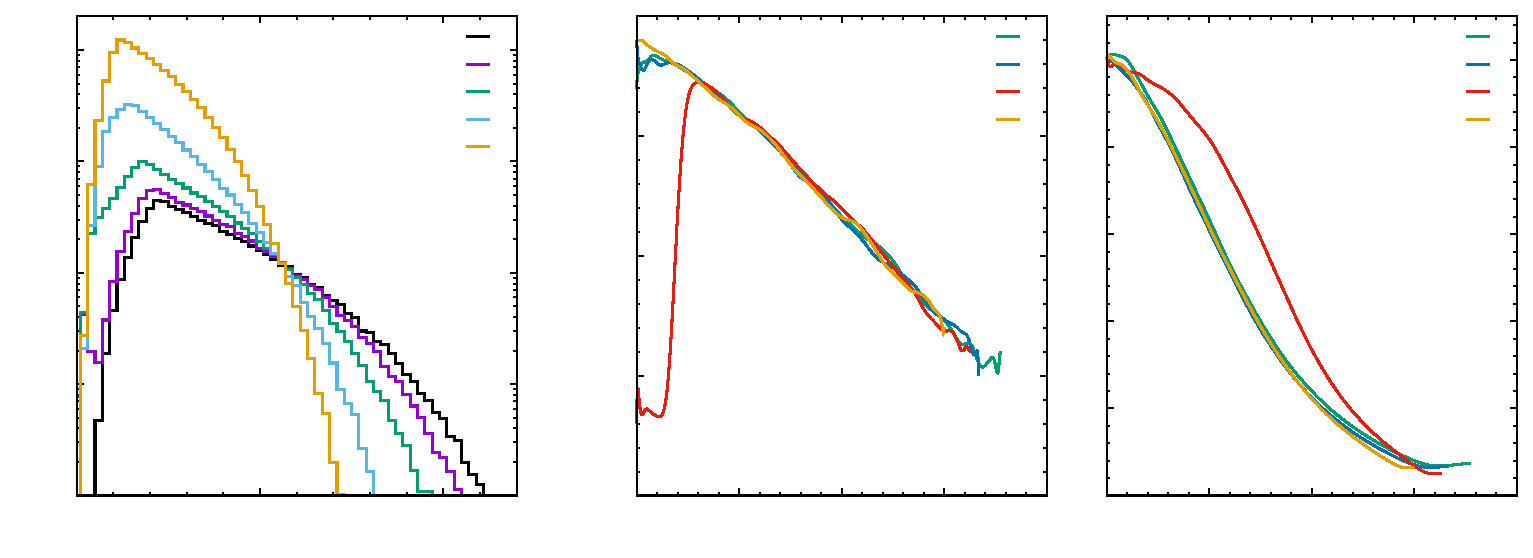
\includegraphics{pics/modmulti}}%
    \gplfronttext
  \end{picture}%
\endgroup
